\chapter{Entrainment detection}
\label{ch:entrainment}

\textbf{Meghavarshini Krishnaswamy, Andrew Wedel, Adam Ussishkin, Cheonkam Jeong} 
\section{Introduction}

    Entrainment (also referred to as `synchronization', `coordination', or `alignment') is the adaption of verbal and non-verbal actions by conversation partners to more closely resemble one another \parencite{borrie2014}. Its role in communication has been described as ``key for supporting important pragmatic aspects of conversation, including taking turns, interaction smoothness, building rapport, fostering social bonds, and maintaining interpersonal relationships''\parencite{borrie2019}. A time-sensitive cooperative task utilizing verbal communication would require participants to optimize their information channel. This makes entrainment a useful metric for assessing the degree of cooperation among teammates, as well as a useful means to assess members' sentiments towards each other, tracking their confidence in the task goals and plans, and identifying team cohesion and bonding over time.

    In speech, entrainment has been observed and analysed using speech rhythm and
    timing, pitch, MFCCs and formant analysis \parencite{reichel2018prosodic,borrie2019syncing}. Speech entrainment occurs in correlation with entrainment at other linguistic levels such as an increase in shared vocabulary and sentence structures \parencite{rahimi2017entrainment}. While entrainment in multi-party conversations has been researched at the lexical-level and sentence-level, speech entrainment has mostly been restricted to two-party conversations. Work on speech entrainment is further limited by the practical difficulties in identifying speech similarity due to the process of entrainment from similarities from physical factors such as people having similar vocal characteristics, or sharing the same speech channel \parencite{nasir2020}.

    Recent research on vocal entrainment has shifted from regression-based analysis to encoding-based neural networks for a few reasons: to model the non-linear relationship between vocalic features, to capture the complexity and diversity of both entrainment and disentrainment, and to train the model on information relevant to entrainment, while ignoring other factors that cause similarity (such as speaker characteristics and features related to the speech recording channel)\parencite{nasir2020}.


\section{Approach}
    The main assumption for automated entrainment detection is that for a given set of speakers and utterances in a discourse, if entrainment takes place, it is located between two neighbouring utterances from different speakers, while utterances from different time points will not show entrainment. So, the model needs to correctly identify neighbouring pairs of utterances, while ignoring similarities pertaining to speaker and channel characteristics (since they are not a function of entrainment). For a multi-party conversation setting, the model also needs to tell the difference between a pair of entrained utterances, a pair of utterances from the same speaker, and utterances from different speakers that are not neighbours.

    Our approach involves training an replicating the feed-forward encoder model and i-vector modelling for entrainment detection proposed and designed by \citeauthor{nasir2020}, 2020. This model assess triplets of utterances for each speaker arranged as follows: an utterance by a given speaker, the utterance succeeding it spoken by a different speaker (positive match for entrainment), and an utterance from a different location in the discourse uttered by the given speaker (negative match for entrainment). In the training process, positive weights are assigned to entrainment characteristics, while speaker and channel characteristics are assigned negative weights. Thus, we have a classification task: for any two utterances, we ask if they are entrained or not.

    \begin{figure}
    \begin{sidecaption}{Representation of the triplet model proposed by \citeauthor{nasir2020}, 2020 [Pg17]. Here, ``Speaker 1 (anchor)'' and `Speaker 2 (positive)' refer to the site of entrainment, while `negative' refers to a non-entrainment utterance}
    \centering
    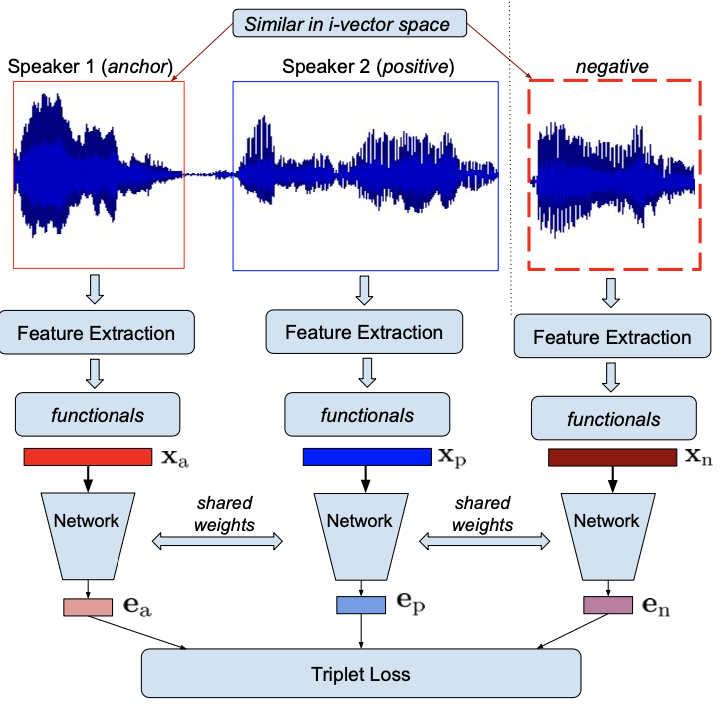
\includegraphics[width=0.6\textwidth]{images/triplet-model.png}
    \label{fig:sentiment_model_schematics}
    \end{sidecaption}
    \end{figure}

    We will utilize the following data and labels from Study-3:
            \begin{itemize}               
                   \item Audio recording
                    Transcript
                   \item Participant demographic information
                   \item Self-evaluation
                   \item MinecraftEntity\_Observation\_Asr\_Speechanalyzer
                   \item MinecraftEntity\_Observation\_Audio\_Speechanalyzer
                   \item MinecraftEntity\_Event\_Dialogue\_Event\_Dialogagent
            \end{itemize}
        % \item Our objectives (in decreasing order of priority):
        %     \begin{itemize} 
        %         \item Build a working statistical model for assessing entrainment while utilizing the vocalic features extracted by the ToMCAT-speechanalyzer system.         
        %         \item Train an encoding-based model using the methodology outlined in \textcite{nasir2020} for a simple classification task that identifies entrainment and directionality in a given conversation.
        %         \item Assess if the current Speechanalyzer system is set up to study entrainment trends as a time series. 
        %     \end{itemize} 

\section{Evaluation}

    Assessing entrainment involves calculating a similarity (or dissimilarity) measure between two utterances from the entrainment category, and observing if this metric of similarity increases or decreases as the speakers continue communicating. For this objective, accuracy scores for the classification task outlined above will be used to measure the performance of the entrainment detector. Because ASIST-ToMCAT is a multi-party conversation, we will examine the process of setting up new baselines for entrainment detection that can account for differences in team dynamics, reflected in how much each speaker talks, and how much other speakers respond to them.  

    We will also explore methods to evaluate two types of entrainment:

    \begin{itemize}
        \item Localized entrainment: Are there observable similarities between utterances by different speakers that occurred next to each other than utterances at different points in time?
        \item Global entrainment: after a given period of objective-oriented speech, is the speech from the conversation aligned more closely? 
    \end{itemize}

    In order to account for ASR errors in the automatically generated transcripts, we will create a corpus of human-generated gold transcriptions. From this corpus, a subsection of the data will be used to identify utterances separated by 50ms pauses, in order to assess any differences in performances due to ASR issues. A manual evaluation of the speech data will also be conducted to examine other environmental noise, so as to account for qualitative differences between the recording conditions of the pristine training data and the real-time ToMCAT speech data. 

   \section{Other Qualitative Assessments}

   Since speech entrainment in conversational setups is a feature of speaker bonding and closeness, it is useful to assess if it co-occurs with positive emotions in spoken statements, lower stress, and higher confidence in the plan and team actions in a co-operative goal-oriented setting. We will utilise the human-generated gold transcriptions as well as manual annotations for emotion and dialogue acts to qualitatively assess if entrainment co-occurs with positive emotions and the acts of sharing information, as well as the relationship between global entrainment and levels of stress and uncertainty. We will also examine if the directionality of entrainment (towards or away from any of the participants) is affected by members' personality or socio-cultural differences, in order to account for natural differences known to impact conversation styles.

